\documentclass[]{article}
\usepackage{lmodern}
\usepackage{amssymb,amsmath}
\usepackage{ifxetex,ifluatex}
\usepackage{fixltx2e} % provides \textsubscript
\ifnum 0\ifxetex 1\fi\ifluatex 1\fi=0 % if pdftex
  \usepackage[T1]{fontenc}
  \usepackage[utf8]{inputenc}
\else % if luatex or xelatex
  \ifxetex
    \usepackage{mathspec}
  \else
    \usepackage{fontspec}
  \fi
  \defaultfontfeatures{Ligatures=TeX,Scale=MatchLowercase}
  \newcommand{\euro}{€}
\fi
% use upquote if available, for straight quotes in verbatim environments
\IfFileExists{upquote.sty}{\usepackage{upquote}}{}
% use microtype if available
\IfFileExists{microtype.sty}{%
\usepackage{microtype}
\UseMicrotypeSet[protrusion]{basicmath} % disable protrusion for tt fonts
}{}
\usepackage[margin=1in]{geometry}
\usepackage{hyperref}
\PassOptionsToPackage{usenames,dvipsnames}{color} % color is loaded by hyperref
\hypersetup{unicode=true,
            pdftitle={Data Manipulation in R},
            pdfborder={0 0 0},
            breaklinks=true}
\urlstyle{same}  % don't use monospace font for urls
\usepackage{color}
\usepackage{fancyvrb}
\newcommand{\VerbBar}{|}
\newcommand{\VERB}{\Verb[commandchars=\\\{\}]}
\DefineVerbatimEnvironment{Highlighting}{Verbatim}{commandchars=\\\{\}}
% Add ',fontsize=\small' for more characters per line
\usepackage{framed}
\definecolor{shadecolor}{RGB}{248,248,248}
\newenvironment{Shaded}{\begin{snugshade}}{\end{snugshade}}
\newcommand{\KeywordTok}[1]{\textcolor[rgb]{0.13,0.29,0.53}{\textbf{{#1}}}}
\newcommand{\DataTypeTok}[1]{\textcolor[rgb]{0.13,0.29,0.53}{{#1}}}
\newcommand{\DecValTok}[1]{\textcolor[rgb]{0.00,0.00,0.81}{{#1}}}
\newcommand{\BaseNTok}[1]{\textcolor[rgb]{0.00,0.00,0.81}{{#1}}}
\newcommand{\FloatTok}[1]{\textcolor[rgb]{0.00,0.00,0.81}{{#1}}}
\newcommand{\ConstantTok}[1]{\textcolor[rgb]{0.00,0.00,0.00}{{#1}}}
\newcommand{\CharTok}[1]{\textcolor[rgb]{0.31,0.60,0.02}{{#1}}}
\newcommand{\SpecialCharTok}[1]{\textcolor[rgb]{0.00,0.00,0.00}{{#1}}}
\newcommand{\StringTok}[1]{\textcolor[rgb]{0.31,0.60,0.02}{{#1}}}
\newcommand{\VerbatimStringTok}[1]{\textcolor[rgb]{0.31,0.60,0.02}{{#1}}}
\newcommand{\SpecialStringTok}[1]{\textcolor[rgb]{0.31,0.60,0.02}{{#1}}}
\newcommand{\ImportTok}[1]{{#1}}
\newcommand{\CommentTok}[1]{\textcolor[rgb]{0.56,0.35,0.01}{\textit{{#1}}}}
\newcommand{\DocumentationTok}[1]{\textcolor[rgb]{0.56,0.35,0.01}{\textbf{\textit{{#1}}}}}
\newcommand{\AnnotationTok}[1]{\textcolor[rgb]{0.56,0.35,0.01}{\textbf{\textit{{#1}}}}}
\newcommand{\CommentVarTok}[1]{\textcolor[rgb]{0.56,0.35,0.01}{\textbf{\textit{{#1}}}}}
\newcommand{\OtherTok}[1]{\textcolor[rgb]{0.56,0.35,0.01}{{#1}}}
\newcommand{\FunctionTok}[1]{\textcolor[rgb]{0.00,0.00,0.00}{{#1}}}
\newcommand{\VariableTok}[1]{\textcolor[rgb]{0.00,0.00,0.00}{{#1}}}
\newcommand{\ControlFlowTok}[1]{\textcolor[rgb]{0.13,0.29,0.53}{\textbf{{#1}}}}
\newcommand{\OperatorTok}[1]{\textcolor[rgb]{0.81,0.36,0.00}{\textbf{{#1}}}}
\newcommand{\BuiltInTok}[1]{{#1}}
\newcommand{\ExtensionTok}[1]{{#1}}
\newcommand{\PreprocessorTok}[1]{\textcolor[rgb]{0.56,0.35,0.01}{\textit{{#1}}}}
\newcommand{\AttributeTok}[1]{\textcolor[rgb]{0.77,0.63,0.00}{{#1}}}
\newcommand{\RegionMarkerTok}[1]{{#1}}
\newcommand{\InformationTok}[1]{\textcolor[rgb]{0.56,0.35,0.01}{\textbf{\textit{{#1}}}}}
\newcommand{\WarningTok}[1]{\textcolor[rgb]{0.56,0.35,0.01}{\textbf{\textit{{#1}}}}}
\newcommand{\AlertTok}[1]{\textcolor[rgb]{0.94,0.16,0.16}{{#1}}}
\newcommand{\ErrorTok}[1]{\textcolor[rgb]{0.64,0.00,0.00}{\textbf{{#1}}}}
\newcommand{\NormalTok}[1]{{#1}}
\usepackage{longtable,booktabs}
\usepackage{graphicx,grffile}
\makeatletter
\def\maxwidth{\ifdim\Gin@nat@width>\linewidth\linewidth\else\Gin@nat@width\fi}
\def\maxheight{\ifdim\Gin@nat@height>\textheight\textheight\else\Gin@nat@height\fi}
\makeatother
% Scale images if necessary, so that they will not overflow the page
% margins by default, and it is still possible to overwrite the defaults
% using explicit options in \includegraphics[width, height, ...]{}
\setkeys{Gin}{width=\maxwidth,height=\maxheight,keepaspectratio}
\setlength{\parindent}{0pt}
\setlength{\parskip}{6pt plus 2pt minus 1pt}
\setlength{\emergencystretch}{3em}  % prevent overfull lines
\providecommand{\tightlist}{%
  \setlength{\itemsep}{0pt}\setlength{\parskip}{0pt}}
\setcounter{secnumdepth}{5}

%%% Use protect on footnotes to avoid problems with footnotes in titles
\let\rmarkdownfootnote\footnote%
\def\footnote{\protect\rmarkdownfootnote}

%%% Change title format to be more compact
\usepackage{titling}

% Create subtitle command for use in maketitle
\newcommand{\subtitle}[1]{
  \posttitle{
    \begin{center}\large#1\end{center}
    }
}

\setlength{\droptitle}{-2em}
  \title{Data Manipulation in R}
  \pretitle{\vspace{\droptitle}\centering\huge}
  \posttitle{\par}
  \author{}
  \preauthor{}\postauthor{}
  \date{}
  \predate{}\postdate{}


% Redefines (sub)paragraphs to behave more like sections
\ifx\paragraph\undefined\else
\let\oldparagraph\paragraph
\renewcommand{\paragraph}[1]{\oldparagraph{#1}\mbox{}}
\fi
\ifx\subparagraph\undefined\else
\let\oldsubparagraph\subparagraph
\renewcommand{\subparagraph}[1]{\oldsubparagraph{#1}\mbox{}}
\fi


\usepackage{amsthm}
\newtheorem{theorem}{Theorem}[section]
\newtheorem{lemma}{Lemma}[section]
\theoremstyle{definition}
\newtheorem{definition}{Definition}[section]
\newtheorem{corollary}{Corollary}[section]
\newtheorem{proposition}{Proposition}[section]
\theoremstyle{definition}
\newtheorem{example}{Example}[section]
\theoremstyle{definition}
\newtheorem{exercise}{Exercise}[section]
\theoremstyle{remark}
\newtheorem*{remark}{Remark}
\newtheorem*{solution}{Solution}
\begin{document}
\maketitle

{
\setcounter{tocdepth}{2}
\tableofcontents
}
\section{Introduction}\label{introduction}

Data manipulation is the process of cleaning, organising and preparing
data in a way that makes it suitable for analysis. Most real-world
datasets require some form of manipulation to facilitate the downstream
analysis and this process is often repeated a number of times during the
data analysis cycle. In this workshop you will learn how to apply a
consistent grammar of data manipulation to raw data and prepare it for
analysis. The following topics are covered in the workshop:

\begin{itemize}
\tightlist
\item
  Learning to use the grammar of data manipulation
\item
  Merging multiple datasets and creating subsets using filters
\item
  Reshaping data between long and wide formats
\item
  Summarising data with group-wise operation
\item
  Setting up data pipelines for efficient data manipulation
\end{itemize}

This workshop is designed for individuals who are already familiar with
R but wish to learn efficient techniques for data manipulation. It is
recommended that you bring your own laptop with the latest version of R
and RStudio installed.

\begin{center}\rule{0.5\linewidth}{\linethickness}\end{center}

\emph{Last Updated: Nov 23, 2017 12:36 AM}

\section{Acknowledgments}\label{acknowledgments}

Content of this workshop is based on the following:

\begin{itemize}
\tightlist
\item
  \href{https://cran.rstudio.com/web/packages/dplyr/vignettes/introduction.html}{Introduction
  to dplyr}
\item
  \href{http://bit.ly/hadley_dplyr_tutorial_2014}{Data manipulation with
  dplyr, 2014}
\item
  \href{https://www.r-bloggers.com/hands-on-dplyr-tutorial-for-faster-data-manipulation-in-r}{Hands-on
  dplyr tutorial for faster data manipulation in R}
\end{itemize}

This work is licensed under a Creative Commons Attribution-ShareAlike
4.0 International License.

\section{Resources}\label{resources}

\begin{itemize}
\item
  \href{http://www.google.com}{Google}
\item
  \href{http://vita.had.co.nz/papers/tidy-data.pdf}{Tidy Data}
\item
  \href{http://tidyverse.org}{Tidyverse}
\item
  \href{https://www.rstudio.com/wp-content/uploads/2015/02/data-wrangling-cheatsheet.pdf}{Data
  Wrangling with dplyr and tidyr Cheat Sheet}
\item
  \href{http://r4ds.had.co.nz}{R for Data Science}
\item
  \href{http://adv-r.had.co.nz}{Advanced R}
\item
  \href{http://bit.ly/hadley_dplyr_tutorial_2014}{Data manipulation with
  dplyr, 2014}
\item
  \href{https://cran.rstudio.com/web/packages/dplyr/vignettes/introduction.html}{Introduction
  to dplyr}
\item
  \href{https://www.r-bloggers.com/hands-on-dplyr-tutorial-for-faster-data-manipulation-in-r}{Hands-on
  dplyr tutorial for faster data manipulation in R}
\end{itemize}

\section{Getting Started}\label{getting-started}

\subsection{Prerequisites}\label{prerequisites}

Basic knowledge of working with datasets in R is essential. This course
assumes that you're comfortable with reading datasets, working with
script files, and navigating in RStudio.

\subsection{Software Requirements}\label{software-requirements}

\subsubsection{R and RStudio}\label{r-and-rstudio}

Recent versions of R (version 3.2 or newer) and RStudio (version 1.0
above) are required.

You can download the latest versions from the links below:

\begin{itemize}
\tightlist
\item
  \href{https://cran.r-project.org}{Download R}
\item
  \href{https://www.rstudio.com/products/rstudio/download}{Download
  RStudio}
\end{itemize}

You can find out the version of R installed by typing \texttt{version}
at the console:

\begin{Shaded}
\begin{Highlighting}[]
\NormalTok{version}
\end{Highlighting}
\end{Shaded}

\begin{verbatim}
               _                           
platform       x86_64-pc-linux-gnu         
arch           x86_64                      
os             linux-gnu                   
system         x86_64, linux-gnu           
status                                     
major          3                           
minor          4.2                         
year           2017                        
month          01                          
day            27                          
svn rev        73369                       
language       R                           
version.string R version 3.4.2 (2017-01-27)
nickname       Short Summer                
\end{verbatim}

\subsection{Required Packages}\label{required-packages}

This workshop relies on three packages: \texttt{dplyr}, \texttt{tidyr},
and \texttt{readr}. There are two ways to install these packages:

\subsubsection{\texorpdfstring{Option 1: Use
\texttt{tidyverse}}{Option 1: Use tidyverse}}\label{option-1-use-tidyverse}

You can either install these two packages individually or use
\texttt{tidyverse}. The \texttt{tidyverse} package is a collection of
packages used for data manipulation and visualization. In addition to
\texttt{dplyr}, \texttt{tidyr}, and \texttt{readr}, it also includes the
following:

\begin{verbatim}
 [1] "broom"       "cli"         "crayon"      "dplyr"       "dbplyr"     
 [6] "forcats"     "ggplot2"     "haven"       "hms"         "httr"       
[11] "jsonlite"    "lubridate"   "magrittr"    "modelr"      "purrr"      
[16] "readr"       "readxl\n(>=" "reprex"      "rlang"       "rstudioapi" 
[21] "rvest"       "stringr"     "tibble"      "tidyr"       "xml2"       
[26] "tidyverse"  
\end{verbatim}

You can install \texttt{tidyverse} using the \texttt{install.packages()}
function:

\begin{Shaded}
\begin{Highlighting}[]
\KeywordTok{install.packages}\NormalTok{(}\StringTok{"tidyverse"}\NormalTok{)}
\end{Highlighting}
\end{Shaded}

You can find out the version of \texttt{tidyverse} installed using the
\texttt{packageVersion()} function:

\begin{Shaded}
\begin{Highlighting}[]
\KeywordTok{packageVersion}\NormalTok{(}\StringTok{"tidyverse"}\NormalTok{)}
\end{Highlighting}
\end{Shaded}

\begin{verbatim}
[1] '1.2.1'
\end{verbatim}

To update \texttt{tidyverse} packages, you can use the
\texttt{tidyverse\_update()} function:

\begin{Shaded}
\begin{Highlighting}[]
\NormalTok{tidyverse::}\KeywordTok{tidyverse_update}\NormalTok{()}
\end{Highlighting}
\end{Shaded}

\subsubsection{Option 2: Install Individual
Packages}\label{option-2-install-individual-packages}

If you encounter any problems installing \texttt{tidyverse}, then the
other option is to install \texttt{dplyr}, \texttt{tidyr}, and
\texttt{readr} individually.

\begin{Shaded}
\begin{Highlighting}[]
\KeywordTok{install.packages}\NormalTok{(}\StringTok{"dplyr"}\NormalTok{)}
\KeywordTok{install.packages}\NormalTok{(}\StringTok{"tidyr"}\NormalTok{)}
\KeywordTok{install.packages}\NormalTok{(}\StringTok{"readr"}\NormalTok{)}
\end{Highlighting}
\end{Shaded}

\section{Basic Operations}\label{basic-operations}

Let's start off by creating a new R script and loading
\texttt{tidyverse}:

\begin{Shaded}
\begin{Highlighting}[]
\KeywordTok{library}\NormalTok{(tidyverse)}
\end{Highlighting}
\end{Shaded}

Clear everything to make sure there's nothing leftover in our
environment

\begin{Shaded}
\begin{Highlighting}[]
\KeywordTok{rm}\NormalTok{(}\DataTypeTok{list =} \KeywordTok{ls}\NormalTok{())}
\end{Highlighting}
\end{Shaded}

\subsection{Data pipelines}\label{data-pipelines}

Dplyr makes it easy to ``chain'' functions together using the
\emph{pipe} operator \texttt{\%\textgreater{}\%}. The following diagram
illustrates the general concept of pipes where data flows from one pipe
to another until all the processing is completed.

\begin{figure}[htbp]
\centering
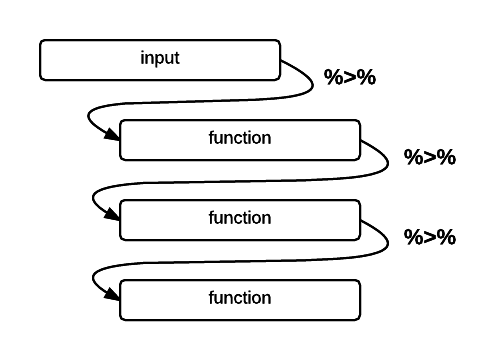
\includegraphics{./img/pipes.png}
\caption{}
\end{figure}

The syntax of the pipe operator \texttt{\%\textgreater{}\%} might appear
unusual at first, but once you get used to it you'll start to appreciate
its power and flexibility.

\subsection{Dataset}\label{dataset}

We're using a dataset of flight departures from Houston in 2011.

\begin{longtable}[c]{@{}ll@{}}
\toprule
Filename & Description\tabularnewline
\midrule
\endhead
flights.csv & Flight departures from Houston in 2011\tabularnewline
weather.csv & Hourly weather\tabularnewline
planes.csv & Metadata for planes\tabularnewline
airports.csv & Metadata for airports\tabularnewline
\bottomrule
\end{longtable}

We're going to use the \texttt{readr} package which provides improved
functions for reading datasets from files. Instead of the usual
\texttt{read.csv()} function, we'll use the \texttt{read\_csv()}
function from \texttt{readr}.

\begin{Shaded}
\begin{Highlighting}[]
\NormalTok{flights <-}\StringTok{ }\KeywordTok{read_csv}\NormalTok{(}\StringTok{"https://raw.githubusercontent.com/altaf-ali/tidydata_tutorial/master/data/flights.csv"}\NormalTok{)}
\NormalTok{weather <-}\StringTok{ }\KeywordTok{read_csv}\NormalTok{(}\StringTok{"https://raw.githubusercontent.com/altaf-ali/tidydata_tutorial/master/data/weather.csv"}\NormalTok{)}
\NormalTok{planes <-}\StringTok{ }\KeywordTok{read_csv}\NormalTok{(}\StringTok{"https://raw.githubusercontent.com/altaf-ali/tidydata_tutorial/master/data/planes.csv"}\NormalTok{)}
\NormalTok{airports <-}\StringTok{ }\KeywordTok{read_csv}\NormalTok{(}\StringTok{"https://raw.githubusercontent.com/altaf-ali/tidydata_tutorial/master/data/airports.csv"}\NormalTok{)}
\end{Highlighting}
\end{Shaded}

Now let's examine the dataset

\begin{Shaded}
\begin{Highlighting}[]
\NormalTok{flights}
\end{Highlighting}
\end{Shaded}

\begin{verbatim}
# A tibble: 227,496 x 14
                  date  hour minute   dep   arr dep_delay arr_delay
                <dttm> <int>  <int> <int> <int>     <int>     <int>
 1 2011-01-01 12:00:00    14      0  1400  1500         0       -10
 2 2011-01-02 12:00:00    14      1  1401  1501         1        -9
 3 2011-01-03 12:00:00    13     52  1352  1502        -8        -8
 4 2011-01-04 12:00:00    14      3  1403  1513         3         3
 5 2011-01-05 12:00:00    14      5  1405  1507         5        -3
 6 2011-01-06 12:00:00    13     59  1359  1503        -1        -7
 7 2011-01-07 12:00:00    13     59  1359  1509        -1        -1
 8 2011-01-08 12:00:00    13     55  1355  1454        -5       -16
 9 2011-01-09 12:00:00    14     43  1443  1554        43        44
10 2011-01-10 12:00:00    14     43  1443  1553        43        43
# ... with 227,486 more rows, and 7 more variables: carrier <chr>,
#   flight <int>, dest <chr>, plane <chr>, cancelled <int>, time <int>,
#   dist <int>
\end{verbatim}

\begin{Shaded}
\begin{Highlighting}[]
\NormalTok{weather}
\end{Highlighting}
\end{Shaded}

\begin{verbatim}
# A tibble: 8,723 x 14
         date  hour  temp dew_point humidity pressure visibility wind_dir
       <date> <int> <dbl>     <dbl>    <int>    <dbl>      <dbl>    <chr>
 1 2011-01-01     0  59.0      28.9       32    29.86         10      NNE
 2 2011-01-01     1  57.2      28.4       33    29.88         10      NNE
 3 2011-01-01     2  55.4      28.4       36    29.93         10      NNW
 4 2011-01-01     3  53.6      28.4       38    29.94         10    North
 5 2011-01-01     4    NA        NA       NA    29.99         10      NNW
 6 2011-01-01     5    NA        NA       NA    30.02         10    North
 7 2011-01-01     6  53.1      17.1       24    30.05         10    North
 8 2011-01-01     7  53.1      16.0       23    30.07         10    North
 9 2011-01-01     8  54.0      18.0       24    30.09         10    North
10 2011-01-01     9  55.4      17.6       23    30.09         10      NNE
# ... with 8,713 more rows, and 6 more variables: wind_dir2 <int>,
#   wind_speed <dbl>, gust_speed <dbl>, precip <dbl>, conditions <chr>,
#   events <chr>
\end{verbatim}

\begin{Shaded}
\begin{Highlighting}[]
\NormalTok{planes}
\end{Highlighting}
\end{Shaded}

\begin{verbatim}
# A tibble: 2,853 x 9
    plane  year               mfr          model no.eng no.seats speed
    <chr> <int>             <chr>          <chr>  <int>    <int> <int>
 1 N576AA  1991 MCDONNELL DOUGLAS DC-9-82(MD-82)      2      172    NA
 2 N557AA  1993        MARZ BARRY      KITFOX IV      1        2    NA
 3 N403AA  1974             RAVEN           S55A     NA        1    60
 4 N492AA  1989 MCDONNELL DOUGLAS DC-9-82(MD-82)      2      172    NA
 5 N262AA  1985 MCDONNELL DOUGLAS DC-9-82(MD-82)      2      172    NA
 6 N493AA  1989 MCDONNELL DOUGLAS DC-9-82(MD-82)      2      172    NA
 7 N477AA  1988 MCDONNELL DOUGLAS DC-9-82(MD-82)      2      172    NA
 8 N476AA  1988 MCDONNELL DOUGLAS DC-9-82(MD-82)      2      172    NA
 9 N504AA    NA AUTHIER ANTHONY P      TIERRA II      1        2    NA
10 N565AA  1987 MCDONNELL DOUGLAS DC-9-83(MD-83)      2      172    NA
# ... with 2,843 more rows, and 2 more variables: engine <chr>, type <chr>
\end{verbatim}

\begin{Shaded}
\begin{Highlighting}[]
\NormalTok{airports}
\end{Highlighting}
\end{Shaded}

\begin{verbatim}
# A tibble: 3,376 x 7
    iata              airport             city state country      lat
   <chr>                <chr>            <chr> <chr>   <chr>    <dbl>
 1   00M              Thigpen      Bay Springs    MS     USA 31.95376
 2   00R Livingston Municipal       Livingston    TX     USA 30.68586
 3   00V          Meadow Lake Colorado Springs    CO     USA 38.94575
 4   01G         Perry-Warsaw            Perry    NY     USA 42.74135
 5   01J     Hilliard Airpark         Hilliard    FL     USA 30.68801
 6   01M    Tishomingo County          Belmont    MS     USA 34.49167
 7   02A           Gragg-Wade          Clanton    AL     USA 32.85049
 8   02C              Capitol       Brookfield    WI     USA 43.08751
 9   02G    Columbiana County   East Liverpool    OH     USA 40.67331
10   03D     Memphis Memorial          Memphis    MO     USA 40.44726
# ... with 3,366 more rows, and 1 more variables: long <dbl>
\end{verbatim}

Notice that because we used \texttt{read\_csv()}, the data frame we
received now prints nicely without having to use the \texttt{head()}
function and does not clutter your screen.

\subsection{Select}\label{select}

The \texttt{select} function is used to select columns.

\begin{itemize}
\tightlist
\item
  Select the destination, duration and distance columns (\texttt{dest},
  \texttt{time} and \texttt{dist})
\end{itemize}

\begin{Shaded}
\begin{Highlighting}[]
\NormalTok{flights %>%}
\StringTok{  }\KeywordTok{select}\NormalTok{(dest, time, dist)}
\end{Highlighting}
\end{Shaded}

\begin{verbatim}
# A tibble: 227,496 x 3
    dest  time  dist
   <chr> <int> <int>
 1   DFW    40   224
 2   DFW    45   224
 3   DFW    48   224
 4   DFW    39   224
 5   DFW    44   224
 6   DFW    45   224
 7   DFW    43   224
 8   DFW    40   224
 9   DFW    41   224
10   DFW    45   224
# ... with 227,486 more rows
\end{verbatim}

Add the arrival delay (\texttt{arr\_delay}) and departure delay
(\texttt{dep\_delay}) columns as well.

\begin{Shaded}
\begin{Highlighting}[]
\NormalTok{flights %>%}
\StringTok{  }\KeywordTok{select}\NormalTok{(dest, time, dist, arr_delay, dep_delay)}
\end{Highlighting}
\end{Shaded}

\begin{verbatim}
# A tibble: 227,496 x 5
    dest  time  dist arr_delay dep_delay
   <chr> <int> <int>     <int>     <int>
 1   DFW    40   224       -10         0
 2   DFW    45   224        -9         1
 3   DFW    48   224        -8        -8
 4   DFW    39   224         3         3
 5   DFW    44   224        -3         5
 6   DFW    45   224        -7        -1
 7   DFW    43   224        -1        -1
 8   DFW    40   224       -16        -5
 9   DFW    41   224        44        43
10   DFW    45   224        43        43
# ... with 227,486 more rows
\end{verbatim}

Other ways to do the same

\begin{Shaded}
\begin{Highlighting}[]
\NormalTok{flights %>%}
\StringTok{  }\KeywordTok{select}\NormalTok{(dest, time, dist, }\KeywordTok{ends_with}\NormalTok{(}\StringTok{"delay"}\NormalTok{))}
\end{Highlighting}
\end{Shaded}

\begin{verbatim}
# A tibble: 227,496 x 5
    dest  time  dist dep_delay arr_delay
   <chr> <int> <int>     <int>     <int>
 1   DFW    40   224         0       -10
 2   DFW    45   224         1        -9
 3   DFW    48   224        -8        -8
 4   DFW    39   224         3         3
 5   DFW    44   224         5        -3
 6   DFW    45   224        -1        -7
 7   DFW    43   224        -1        -1
 8   DFW    40   224        -5       -16
 9   DFW    41   224        43        44
10   DFW    45   224        43        43
# ... with 227,486 more rows
\end{verbatim}

and \ldots{}

\begin{Shaded}
\begin{Highlighting}[]
\NormalTok{flights %>%}
\StringTok{  }\KeywordTok{select}\NormalTok{(dest, time, dist, }\KeywordTok{contains}\NormalTok{(}\StringTok{"delay"}\NormalTok{))}
\end{Highlighting}
\end{Shaded}

\begin{verbatim}
# A tibble: 227,496 x 5
    dest  time  dist dep_delay arr_delay
   <chr> <int> <int>     <int>     <int>
 1   DFW    40   224         0       -10
 2   DFW    45   224         1        -9
 3   DFW    48   224        -8        -8
 4   DFW    39   224         3         3
 5   DFW    44   224         5        -3
 6   DFW    45   224        -1        -7
 7   DFW    43   224        -1        -1
 8   DFW    40   224        -5       -16
 9   DFW    41   224        43        44
10   DFW    45   224        43        43
# ... with 227,486 more rows
\end{verbatim}

Select all columns from \texttt{date} to \texttt{arr}

\begin{Shaded}
\begin{Highlighting}[]
\NormalTok{flights %>%}
\StringTok{  }\KeywordTok{select}\NormalTok{(date:arr)}
\end{Highlighting}
\end{Shaded}

\begin{verbatim}
# A tibble: 227,496 x 5
                  date  hour minute   dep   arr
                <dttm> <int>  <int> <int> <int>
 1 2011-01-01 12:00:00    14      0  1400  1500
 2 2011-01-02 12:00:00    14      1  1401  1501
 3 2011-01-03 12:00:00    13     52  1352  1502
 4 2011-01-04 12:00:00    14      3  1403  1513
 5 2011-01-05 12:00:00    14      5  1405  1507
 6 2011-01-06 12:00:00    13     59  1359  1503
 7 2011-01-07 12:00:00    13     59  1359  1509
 8 2011-01-08 12:00:00    13     55  1355  1454
 9 2011-01-09 12:00:00    14     43  1443  1554
10 2011-01-10 12:00:00    14     43  1443  1553
# ... with 227,486 more rows
\end{verbatim}

Select all \emph{except} \texttt{plane} column using the \emph{minus}
sign

\begin{Shaded}
\begin{Highlighting}[]
\NormalTok{flights %>%}
\StringTok{  }\KeywordTok{select}\NormalTok{(-plane)}
\end{Highlighting}
\end{Shaded}

\begin{verbatim}
# A tibble: 227,496 x 13
                  date  hour minute   dep   arr dep_delay arr_delay
                <dttm> <int>  <int> <int> <int>     <int>     <int>
 1 2011-01-01 12:00:00    14      0  1400  1500         0       -10
 2 2011-01-02 12:00:00    14      1  1401  1501         1        -9
 3 2011-01-03 12:00:00    13     52  1352  1502        -8        -8
 4 2011-01-04 12:00:00    14      3  1403  1513         3         3
 5 2011-01-05 12:00:00    14      5  1405  1507         5        -3
 6 2011-01-06 12:00:00    13     59  1359  1503        -1        -7
 7 2011-01-07 12:00:00    13     59  1359  1509        -1        -1
 8 2011-01-08 12:00:00    13     55  1355  1454        -5       -16
 9 2011-01-09 12:00:00    14     43  1443  1554        43        44
10 2011-01-10 12:00:00    14     43  1443  1553        43        43
# ... with 227,486 more rows, and 6 more variables: carrier <chr>,
#   flight <int>, dest <chr>, cancelled <int>, time <int>, dist <int>
\end{verbatim}

\subsection{Filter}\label{filter}

The \texttt{filter()} function returns rows with matching conditions. We
can find all flights to Boston (BOS) like this:

\begin{Shaded}
\begin{Highlighting}[]
\NormalTok{flights %>%}
\StringTok{  }\KeywordTok{filter}\NormalTok{(dest ==}\StringTok{ "BOS"}\NormalTok{)}
\end{Highlighting}
\end{Shaded}

\begin{verbatim}
# A tibble: 1,752 x 14
                  date  hour minute   dep   arr dep_delay arr_delay
                <dttm> <int>  <int> <int> <int>     <int>     <int>
 1 2011-01-31 12:00:00     7     35   735  1220         0         4
 2 2011-01-31 12:00:00    10     47  1047  1526        -3        -5
 3 2011-01-31 12:00:00    13      5  1305  1746         0        -3
 4 2011-01-31 12:00:00    19      1  1901  2332         6        -1
 5 2011-01-31 12:00:00    15     50  1550  2012         0       -25
 6 2011-01-30 12:00:00    10     46  1046  1518        -4        -8
 7 2011-01-30 12:00:00    13     19  1319  1811        14        22
 8 2011-01-30 12:00:00    19      9  1909    23        14        50
 9 2011-01-30 12:00:00    15     53  1553  2030         3        -7
10 2011-01-29 12:00:00     7     40   740  1227         5        16
# ... with 1,742 more rows, and 7 more variables: carrier <chr>,
#   flight <int>, dest <chr>, plane <chr>, cancelled <int>, time <int>,
#   dist <int>
\end{verbatim}

Let's build on the previous exercise and find all flights to Boston
(BOS) and select only the \texttt{dest}, \texttt{time}, \texttt{dist}
columns:

\begin{Shaded}
\begin{Highlighting}[]
\NormalTok{flights %>%}
\StringTok{  }\KeywordTok{select}\NormalTok{(dest, time, dist) %>%}
\StringTok{  }\KeywordTok{filter}\NormalTok{(dest ==}\StringTok{ "BOS"}\NormalTok{)}
\end{Highlighting}
\end{Shaded}

\begin{verbatim}
# A tibble: 1,752 x 3
    dest  time  dist
   <chr> <int> <int>
 1   BOS   195  1597
 2   BOS   188  1597
 3   BOS   190  1597
 4   BOS   188  1597
 5   BOS   180  1597
 6   BOS   190  1597
 7   BOS   185  1597
 8   BOS   198  1597
 9   BOS   194  1597
10   BOS   203  1597
# ... with 1,742 more rows
\end{verbatim}

Now let's do the filter first and then select the columns

\begin{Shaded}
\begin{Highlighting}[]
\NormalTok{flights %>%}
\StringTok{  }\KeywordTok{filter}\NormalTok{(dest ==}\StringTok{ "BOS"}\NormalTok{) %>%}
\StringTok{  }\KeywordTok{select}\NormalTok{(dest, time, dist) }
\end{Highlighting}
\end{Shaded}

\begin{verbatim}
# A tibble: 1,752 x 3
    dest  time  dist
   <chr> <int> <int>
 1   BOS   195  1597
 2   BOS   188  1597
 3   BOS   190  1597
 4   BOS   188  1597
 5   BOS   180  1597
 6   BOS   190  1597
 7   BOS   185  1597
 8   BOS   198  1597
 9   BOS   194  1597
10   BOS   203  1597
# ... with 1,742 more rows
\end{verbatim}

In this case the order doesn't matter, but when using pipes make sure
you understand that each function is executed in sequence and the
results are then fed to the next one.

\subsubsection{Exercise}\label{exercise}

Find all flights that match the following conditions:

\begin{enumerate}
\def\labelenumi{\arabic{enumi}.}
\tightlist
\item
  To SFO or OAK
\item
  In January
\item
  Delayed by more than an hour
\item
  Departed between midnight and 5am
\item
  Arrival delay more than twice the departure delay
\end{enumerate}

Here's a brief summary of operators you can use:

\textbf{Comparison Operators}

\begin{tabular}{l|l|l|l}
\hline
Operator & Description & Example (assume x is 5) & Result\\
\hline
> & greater than & x > 5 & FALSE\\
\hline
>= & greater than or equal to & x >= 5 & TRUE\\
\hline
< & less than & x < 5 & FALSE\\
\hline
<= & less than or equal to & x <= 5 & TRUE\\
\hline
== & equal to & x == 5 & TRUE\\
\hline
!= & not equal to & x != 5 & FALSE\\
\hline
\end{tabular}

\textbf{Logical Operators}

\begin{tabular}{l|l}
\hline
Operator & Description\\
\hline
! & not\\
\hline
| & or\\
\hline
\& & and\\
\hline
\end{tabular}

\textbf{Other Operators}

\begin{tabular}{l|l|l|l}
\hline
Operator & Description & Example (assume x is 5) & Result\\
\hline
\%in\% & check element in a vector & x \%in\% c(1, 3, 5, 7)<br>x \%in\% c(2, 4, 6, 8) & TRUE<br>FALSE\\
\hline
\end{tabular}

\subsection{Arrange}\label{arrange}

The \texttt{arrange()} function is used to sort the rows based on one or
more columns

\begin{Shaded}
\begin{Highlighting}[]
\NormalTok{flights %>%}
\StringTok{  }\KeywordTok{arrange}\NormalTok{(dest)}
\end{Highlighting}
\end{Shaded}

\begin{verbatim}
# A tibble: 227,496 x 14
                  date  hour minute   dep   arr dep_delay arr_delay
                <dttm> <int>  <int> <int> <int>     <int>     <int>
 1 2011-01-31 12:00:00    17     33  1733  1901        -2        -4
 2 2011-01-30 12:00:00    17     50  1750  1913        15         8
 3 2011-01-29 12:00:00    17     32  1732  1837        -3       -23
 4 2011-01-28 12:00:00    17     33  1733  1848        -2       -17
 5 2011-01-27 12:00:00    17     41  1741  1854         6       -11
 6 2011-01-26 12:00:00    17     32  1732  1853        -3       -12
 7 2011-01-25 12:00:00    17     29  1729  1858        -6        -7
 8 2011-01-24 12:00:00    17     34  1734  1845        -1       -20
 9 2011-01-23 12:00:00    17     35  1735  1853         0       -12
10 2011-01-22 12:00:00    17     33  1733  1843        -2       -17
# ... with 227,486 more rows, and 7 more variables: carrier <chr>,
#   flight <int>, dest <chr>, plane <chr>, cancelled <int>, time <int>,
#   dist <int>
\end{verbatim}

\subsubsection{Exercise}\label{exercise-1}

\begin{enumerate}
\def\labelenumi{\arabic{enumi}.}
\tightlist
\item
  Order flights by departure date and time
\item
  Which flights were most delayed?
\item
  Which flights caught up the most time during flight?
\end{enumerate}

\subsection{Mutate}\label{mutate}

The \texttt{mutate()} function is used to create new variables.

Up until now we've only been examining the dataset but haven't made any
changes to it. All our functions so far have simply displayed the
results on screen but haven't created or modified existing variables.
Let's see how we can create a new variable called \texttt{speed} based
on the distance and duration in the flights dataframe.

In this exercise we're adding a new variable to an existing dataframe so
we'll just overwrite the \texttt{flights} variable with the one that has
a \texttt{speed} column

\begin{Shaded}
\begin{Highlighting}[]
\NormalTok{flights <-}\StringTok{ }\NormalTok{flights %>%}
\StringTok{  }\KeywordTok{mutate}\NormalTok{(}\DataTypeTok{speed =} \NormalTok{dist /}\StringTok{ }\NormalTok{(time /}\StringTok{ }\DecValTok{60}\NormalTok{))}
\end{Highlighting}
\end{Shaded}

\subsubsection{Exercise}\label{exercise-2}

\begin{enumerate}
\def\labelenumi{\arabic{enumi}.}
\tightlist
\item
  Add a variable to show how much time was made up (or lost) during
  flight
\end{enumerate}

\subsection{Summarise}\label{summarise}

Let's count the number of flights departing each day.

\begin{Shaded}
\begin{Highlighting}[]
\NormalTok{flights %>%}
\StringTok{  }\KeywordTok{group_by}\NormalTok{(date) %>%}
\StringTok{  }\KeywordTok{summarise}\NormalTok{(}\DataTypeTok{count =} \KeywordTok{n}\NormalTok{()) }
\end{Highlighting}
\end{Shaded}

\begin{verbatim}
# A tibble: 365 x 2
                  date count
                <dttm> <int>
 1 2011-01-01 12:00:00   552
 2 2011-01-02 12:00:00   678
 3 2011-01-03 12:00:00   702
 4 2011-01-04 12:00:00   583
 5 2011-01-05 12:00:00   590
 6 2011-01-06 12:00:00   660
 7 2011-01-07 12:00:00   661
 8 2011-01-08 12:00:00   500
 9 2011-01-09 12:00:00   602
10 2011-01-10 12:00:00   659
# ... with 355 more rows
\end{verbatim}

Here's a nice little trick. You can use \texttt{View()} to look at the
results of a pipe operation without creating new variables.

\begin{Shaded}
\begin{Highlighting}[]
\NormalTok{flights %>%}
\StringTok{  }\KeywordTok{group_by}\NormalTok{(date) %>%}
\StringTok{  }\KeywordTok{summarise}\NormalTok{(}\DataTypeTok{count =} \KeywordTok{n}\NormalTok{()) %>%}
\StringTok{  }\KeywordTok{View}\NormalTok{()}
\end{Highlighting}
\end{Shaded}

Of course, often times we'd want to save the summary in a variable for
further analysis.

Let's find the average departure delay for each destination

\begin{Shaded}
\begin{Highlighting}[]
\NormalTok{delays <-}\StringTok{ }\NormalTok{flights %>%}
\StringTok{    }\KeywordTok{group_by}\NormalTok{(dest) %>%}
\StringTok{    }\KeywordTok{summarise}\NormalTok{(}\DataTypeTok{mean =} \KeywordTok{mean}\NormalTok{(dep_delay))}

\NormalTok{delays}
\end{Highlighting}
\end{Shaded}

\begin{verbatim}
# A tibble: 116 x 2
    dest   mean
   <chr>  <dbl>
 1   ABQ     NA
 2   AEX     NA
 3   AGS 10.000
 4   AMA     NA
 5   ANC 24.952
 6   ASE     NA
 7   ATL     NA
 8   AUS     NA
 9   AVL     NA
10   BFL     NA
# ... with 106 more rows
\end{verbatim}

\subsubsection{Exercise}\label{exercise-3}

\begin{enumerate}
\def\labelenumi{\arabic{enumi}.}
\tightlist
\item
  What's wrong with the results above, and how would you fix the
  problem?
\item
  Can you think of using filter to solve the problem?
\item
  Use help to find out two other ways to do summarize/n combination in
  dplyr.
\item
  How many different destinations can you fly to from Houston?
\item
  Which destinations have the highest average delays?
\item
  Which flights (carrier + flight number) happen everyday and where do
  they fly?
\item
  How do delays (of non-cancelled flights) vary over the course of a
  day?
\end{enumerate}

\subsection{Unite}\label{unite}

The \texttt{unite} function is useful for combining multiple columns
together. In the example below, we join the \texttt{carrier} and
\texttt{flight} to create a unique \texttt{flight\_id} column.

\begin{Shaded}
\begin{Highlighting}[]
\NormalTok{flights %>%}
\StringTok{  }\KeywordTok{unite}\NormalTok{(flight_id, carrier, flight, }\DataTypeTok{sep =} \StringTok{"-"}\NormalTok{, }\DataTypeTok{remove =} \OtherTok{FALSE}\NormalTok{) %>%}
\StringTok{  }\KeywordTok{select}\NormalTok{(date, carrier, flight, flight_id)}
\end{Highlighting}
\end{Shaded}

\begin{verbatim}
# A tibble: 227,496 x 4
                  date carrier flight flight_id
 *              <dttm>   <chr>  <int>     <chr>
 1 2011-01-01 12:00:00      AA    428    AA-428
 2 2011-01-02 12:00:00      AA    428    AA-428
 3 2011-01-03 12:00:00      AA    428    AA-428
 4 2011-01-04 12:00:00      AA    428    AA-428
 5 2011-01-05 12:00:00      AA    428    AA-428
 6 2011-01-06 12:00:00      AA    428    AA-428
 7 2011-01-07 12:00:00      AA    428    AA-428
 8 2011-01-08 12:00:00      AA    428    AA-428
 9 2011-01-09 12:00:00      AA    428    AA-428
10 2011-01-10 12:00:00      AA    428    AA-428
# ... with 227,486 more rows
\end{verbatim}

\subsection{Separate}\label{separate}

The \texttt{separate} function works the other way around by splitting a
single column into multiple columns. Let's split the \texttt{date}
column into separate \texttt{date} and \texttt{time} columns.

\begin{Shaded}
\begin{Highlighting}[]
\NormalTok{flights %>%}
\StringTok{  }\KeywordTok{separate}\NormalTok{(date, }\KeywordTok{c}\NormalTok{(}\StringTok{"date"}\NormalTok{, }\StringTok{"time"}\NormalTok{), }\DataTypeTok{sep =} \StringTok{" "}\NormalTok{)}
\end{Highlighting}
\end{Shaded}

\begin{verbatim}
# A tibble: 227,496 x 16
         date     time  hour minute   dep   arr dep_delay arr_delay
 *      <chr>    <chr> <int>  <int> <int> <int>     <int>     <int>
 1 2011-01-01 12:00:00    14      0  1400  1500         0       -10
 2 2011-01-02 12:00:00    14      1  1401  1501         1        -9
 3 2011-01-03 12:00:00    13     52  1352  1502        -8        -8
 4 2011-01-04 12:00:00    14      3  1403  1513         3         3
 5 2011-01-05 12:00:00    14      5  1405  1507         5        -3
 6 2011-01-06 12:00:00    13     59  1359  1503        -1        -7
 7 2011-01-07 12:00:00    13     59  1359  1509        -1        -1
 8 2011-01-08 12:00:00    13     55  1355  1454        -5       -16
 9 2011-01-09 12:00:00    14     43  1443  1554        43        44
10 2011-01-10 12:00:00    14     43  1443  1553        43        43
# ... with 227,486 more rows, and 8 more variables: carrier <chr>,
#   flight <int>, dest <chr>, plane <chr>, cancelled <int>, time <int>,
#   dist <int>, speed <dbl>
\end{verbatim}

\subsubsection{Exercise}\label{exercise-4}

\begin{enumerate}
\def\labelenumi{\arabic{enumi}.}
\tightlist
\item
  Split the \texttt{date} column into \texttt{year}, \texttt{month}, and
  \texttt{day} columns
\item
  Ensure that the \texttt{year}, \texttt{month}, and \texttt{day}
  columns are of type \emph{integer} (NOT \emph{character})

  \begin{itemize}
  \tightlist
  \item
    HINT: Use online help for \texttt{separate} for an easy way to do
    this
  \end{itemize}
\end{enumerate}

\section{Merging Datasets}\label{merging-datasets}

Let's start by loading the \texttt{tidyverse} package

\begin{Shaded}
\begin{Highlighting}[]
\KeywordTok{library}\NormalTok{(tidyverse)}
\end{Highlighting}
\end{Shaded}

Clear everything to make sure there's nothing leftover in our
environment

\begin{Shaded}
\begin{Highlighting}[]
\KeywordTok{rm}\NormalTok{(}\DataTypeTok{list =} \KeywordTok{ls}\NormalTok{())}
\end{Highlighting}
\end{Shaded}

Next, we load three datasets of universities, cities, and states.

\begin{Shaded}
\begin{Highlighting}[]
\NormalTok{universities <-}\StringTok{ }\KeywordTok{read_csv}\NormalTok{(}\StringTok{"https://raw.githubusercontent.com/altaf-ali/tidydata_tutorial/master/data/universities.csv"}\NormalTok{)}
\NormalTok{cities <-}\StringTok{ }\KeywordTok{read_csv}\NormalTok{(}\StringTok{"https://raw.githubusercontent.com/altaf-ali/tidydata_tutorial/master/data/cities.csv"}\NormalTok{)}
\NormalTok{states <-}\StringTok{ }\KeywordTok{read_csv}\NormalTok{(}\StringTok{"https://raw.githubusercontent.com/altaf-ali/tidydata_tutorial/master/data/states.csv"}\NormalTok{)}
\end{Highlighting}
\end{Shaded}

Let's see how we can merge the \texttt{universities} dataset with the
\texttt{cities} dataset.

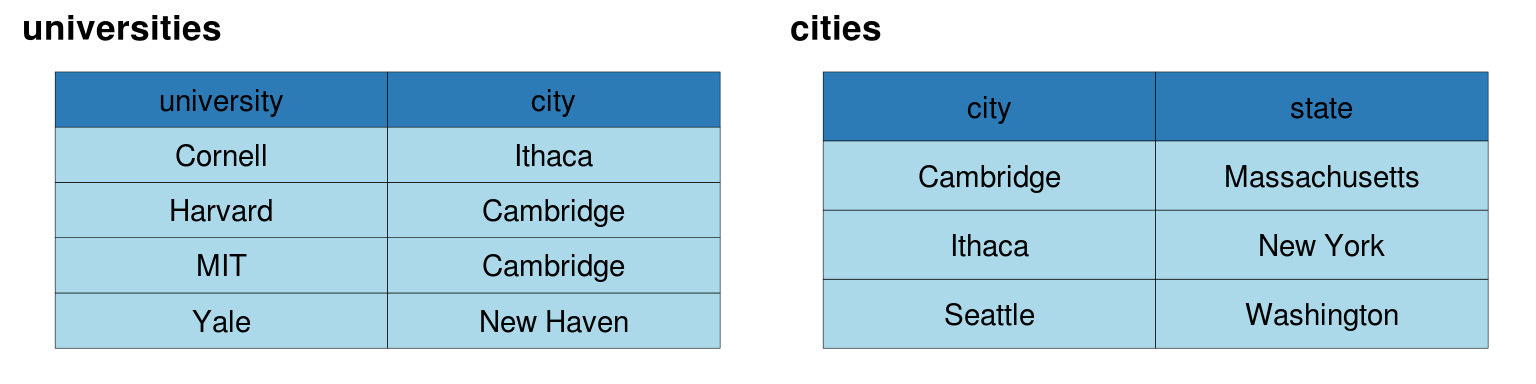
\includegraphics{tidydata_tutorial_files/figure-latex/unnamed-chunk-35-1.pdf}

\subsection{Left Join}\label{left-join}

\begin{Shaded}
\begin{Highlighting}[]
\NormalTok{universities %>%}
\StringTok{  }\KeywordTok{left_join}\NormalTok{(cities, }\DataTypeTok{by =} \StringTok{"city"}\NormalTok{)}
\end{Highlighting}
\end{Shaded}

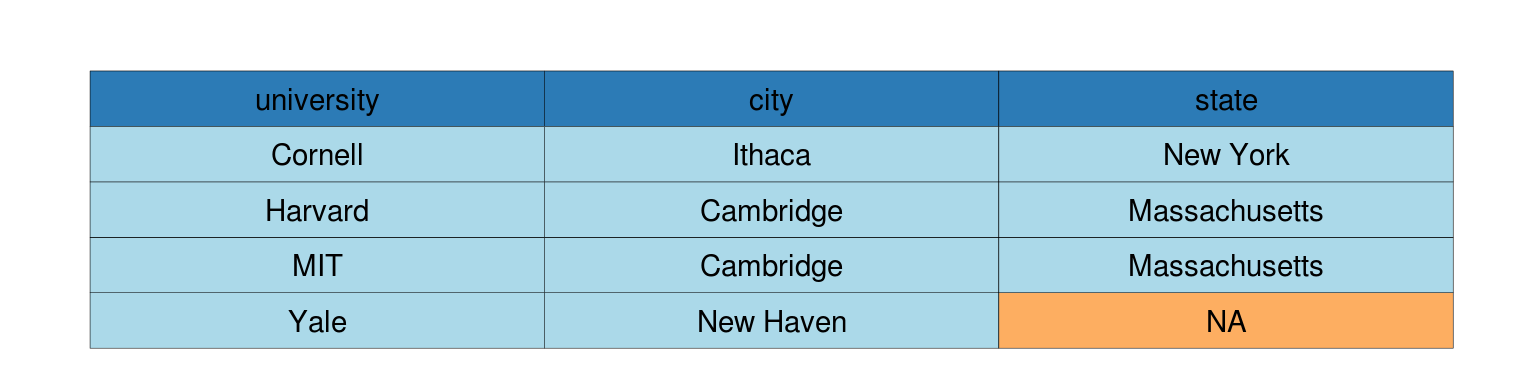
\includegraphics{tidydata_tutorial_files/figure-latex/unnamed-chunk-37-1.pdf}

\subsection{Right Join}\label{right-join}

\begin{Shaded}
\begin{Highlighting}[]
\NormalTok{universities %>%}
\StringTok{  }\KeywordTok{right_join}\NormalTok{(cities, }\DataTypeTok{by =} \StringTok{"city"}\NormalTok{)}
\end{Highlighting}
\end{Shaded}

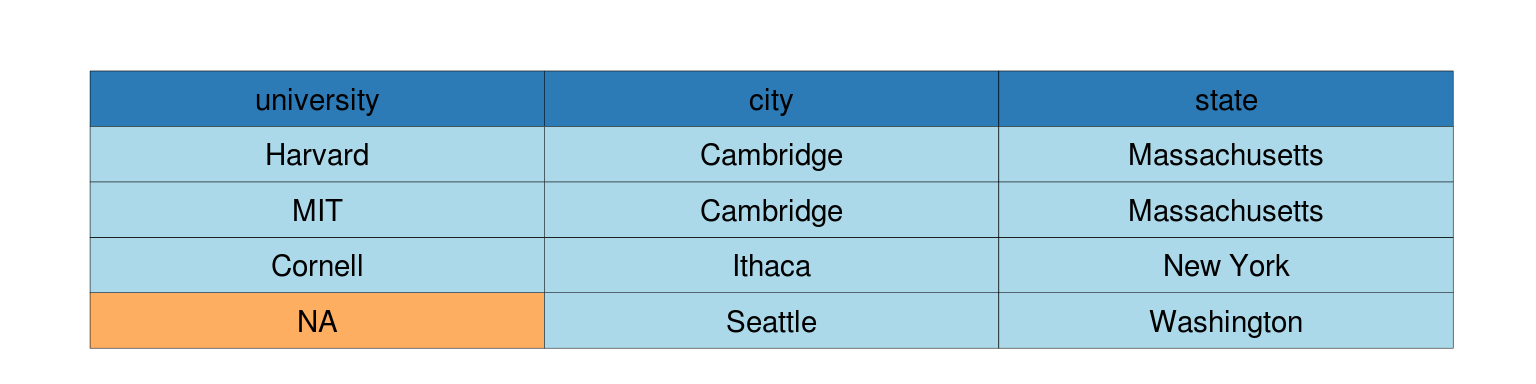
\includegraphics{tidydata_tutorial_files/figure-latex/unnamed-chunk-39-1.pdf}

\subsection{Inner Join}\label{inner-join}

\begin{Shaded}
\begin{Highlighting}[]
\NormalTok{universities %>%}
\StringTok{  }\KeywordTok{inner_join}\NormalTok{(cities, }\DataTypeTok{by =} \StringTok{"city"}\NormalTok{)}
\end{Highlighting}
\end{Shaded}

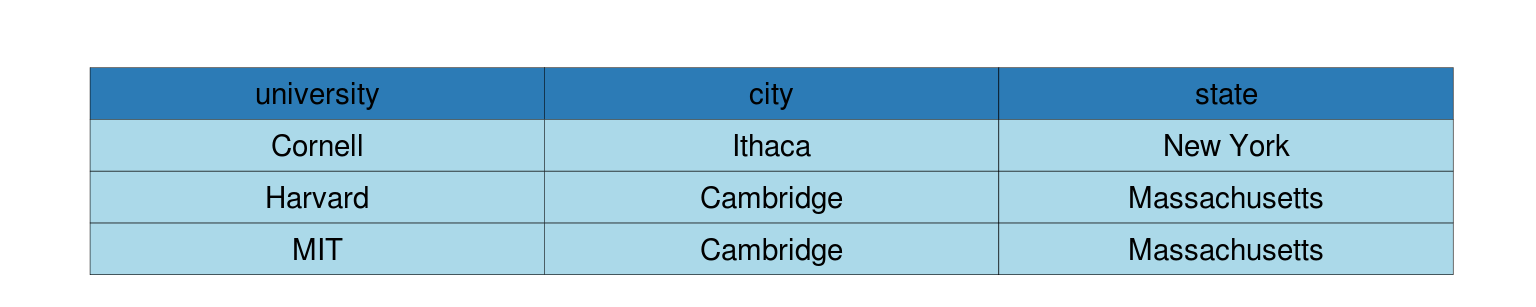
\includegraphics{tidydata_tutorial_files/figure-latex/unnamed-chunk-41-1.pdf}

\subsection{Full Join}\label{full-join}

\begin{Shaded}
\begin{Highlighting}[]
\NormalTok{universities %>%}
\StringTok{  }\KeywordTok{full_join}\NormalTok{(cities, }\DataTypeTok{by =} \StringTok{"city"}\NormalTok{)}
\end{Highlighting}
\end{Shaded}

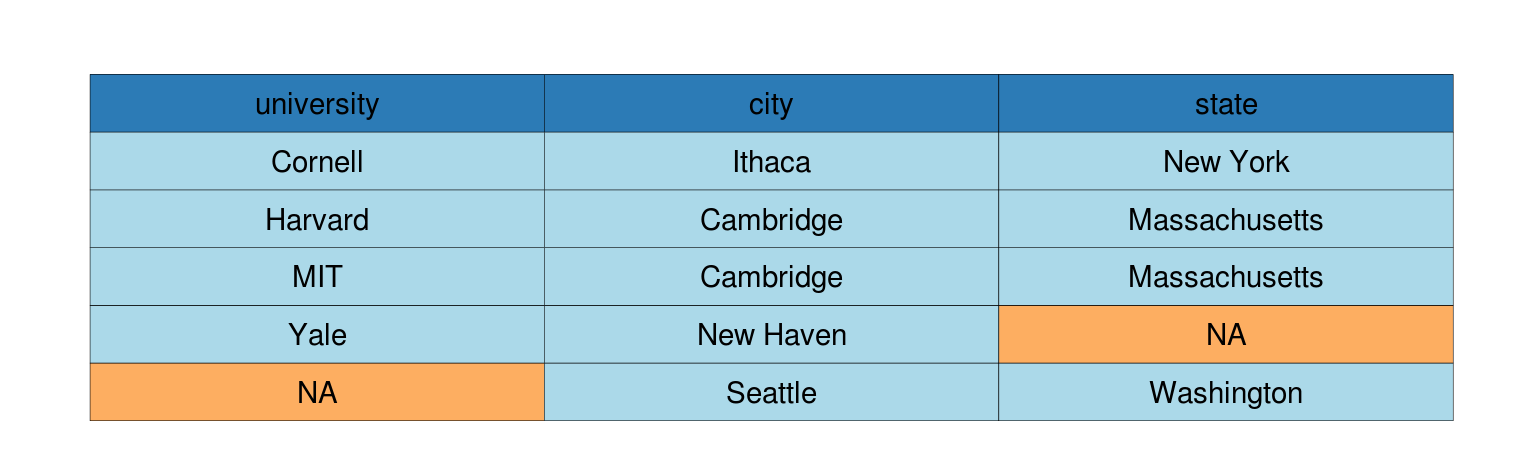
\includegraphics{tidydata_tutorial_files/figure-latex/unnamed-chunk-43-1.pdf}

\subsection{Different Column Names}\label{different-column-names}

In the previous example both our datasets included a column named
\texttt{city}. But what if the names of the columns in the two datasets
were not the same? For example, let's take a look at the \texttt{states}
table:

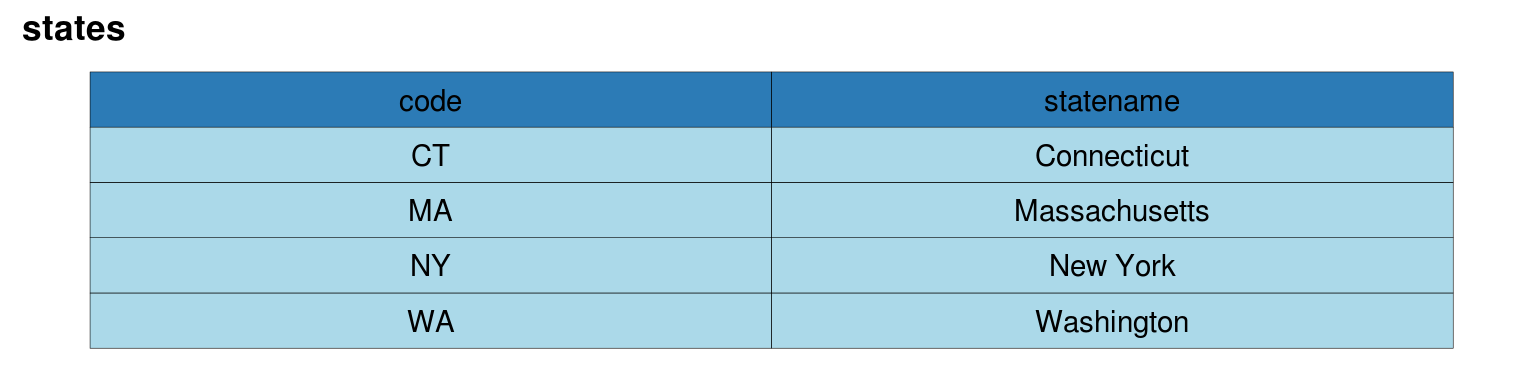
\includegraphics{tidydata_tutorial_files/figure-latex/unnamed-chunk-44-1.pdf}

What if we were to merge the \texttt{cities} dataset with
\texttt{states}?

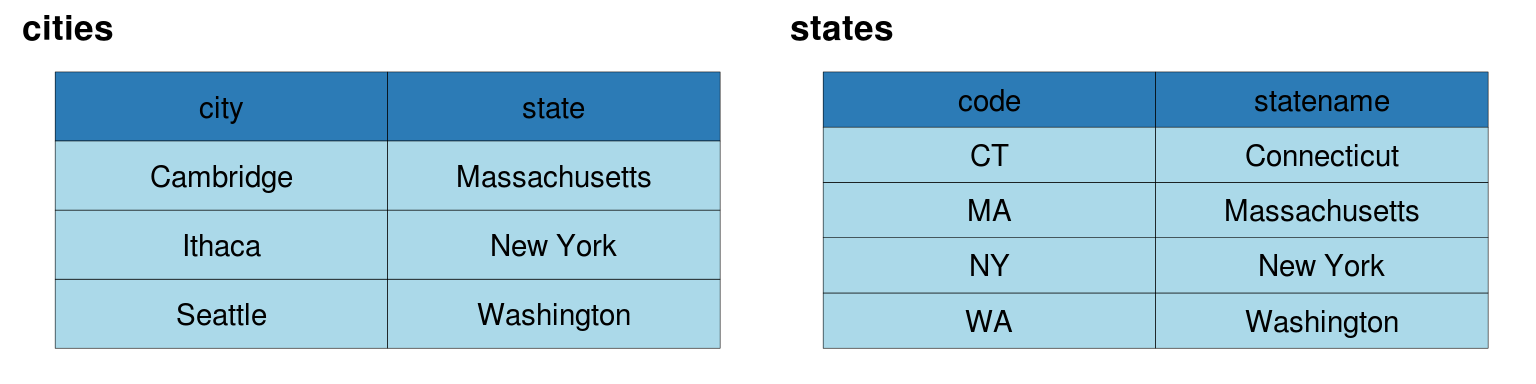
\includegraphics{tidydata_tutorial_files/figure-latex/unnamed-chunk-45-1.pdf}

One option would be to rename the columns so their names would match,
but you don't really need to do that. You can simply tell the join
functions the mapping between the different names.

\begin{Shaded}
\begin{Highlighting}[]
\NormalTok{cities %>%}
\StringTok{  }\KeywordTok{left_join}\NormalTok{(states, }\DataTypeTok{by =} \KeywordTok{c}\NormalTok{(}\StringTok{"state"} \NormalTok{=}\StringTok{ "statename"}\NormalTok{))}
\end{Highlighting}
\end{Shaded}

In the above example, we're telling \texttt{left\_join()} to merge using
the \texttt{state} column from the \texttt{cities} data frame and
\texttt{statename} column from the \texttt{states} data frame.

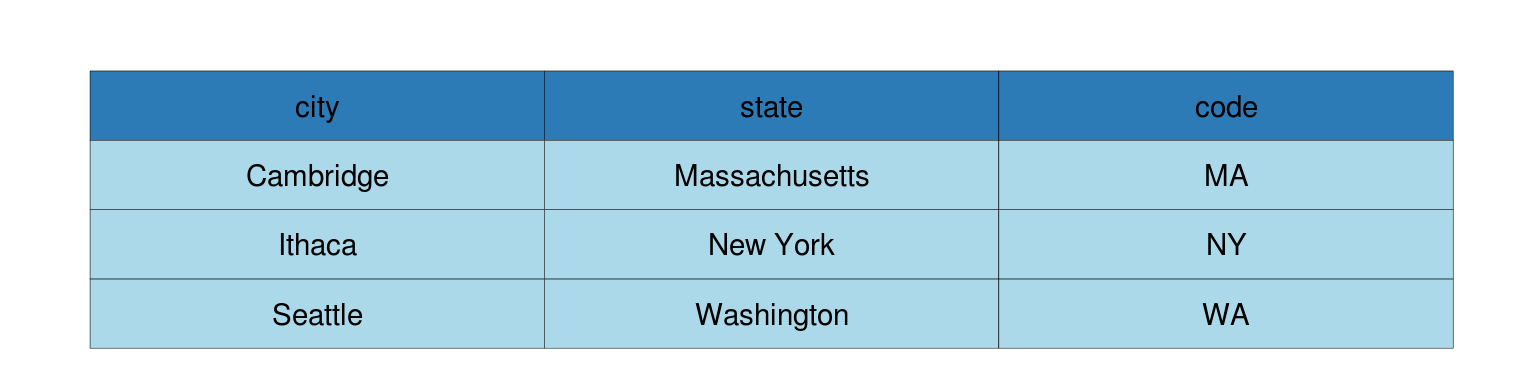
\includegraphics{tidydata_tutorial_files/figure-latex/unnamed-chunk-47-1.pdf}

\subsection{Exercise}\label{exercise-5}

\begin{enumerate}
\def\labelenumi{\arabic{enumi}.}
\item
  Load the following datasets:

\begin{Shaded}
\begin{Highlighting}[]
\NormalTok{presidents <-}\StringTok{ }\KeywordTok{read_csv}\NormalTok{(}\StringTok{"https://raw.githubusercontent.com/altaf-ali/tidydata_tutorial/master/data/presidents.csv"}\NormalTok{)}
\NormalTok{presidents_home <-}\StringTok{ }\KeywordTok{read_csv}\NormalTok{(}\StringTok{"https://raw.githubusercontent.com/altaf-ali/tidydata_tutorial/master/data/presidents_home.csv"}\NormalTok{)}
\end{Highlighting}
\end{Shaded}

  The datasets include names of U.S. presidents:

  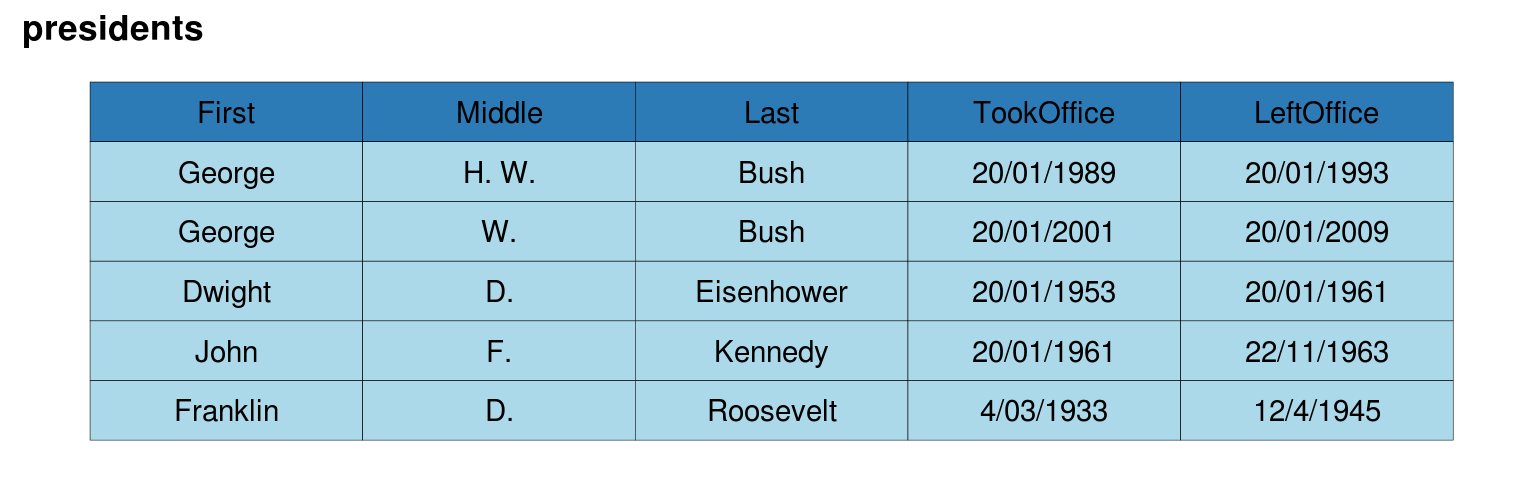
\includegraphics{tidydata_tutorial_files/figure-latex/unnamed-chunk-49-1.pdf}

  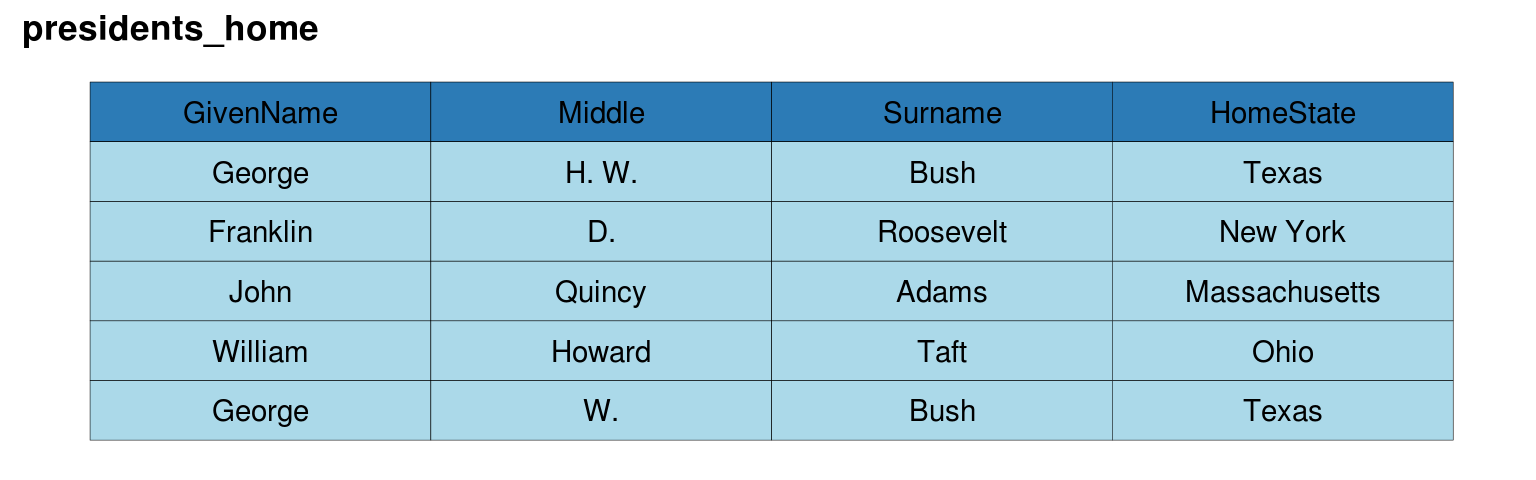
\includegraphics{tidydata_tutorial_files/figure-latex/unnamed-chunk-50-1.pdf}
\item
  Merge the two datasets so that it ONLY includes observations that
  exist in BOTH the datasets. There should be no missing values or
  \texttt{NA} in the merged table. The results should match the
  following:

  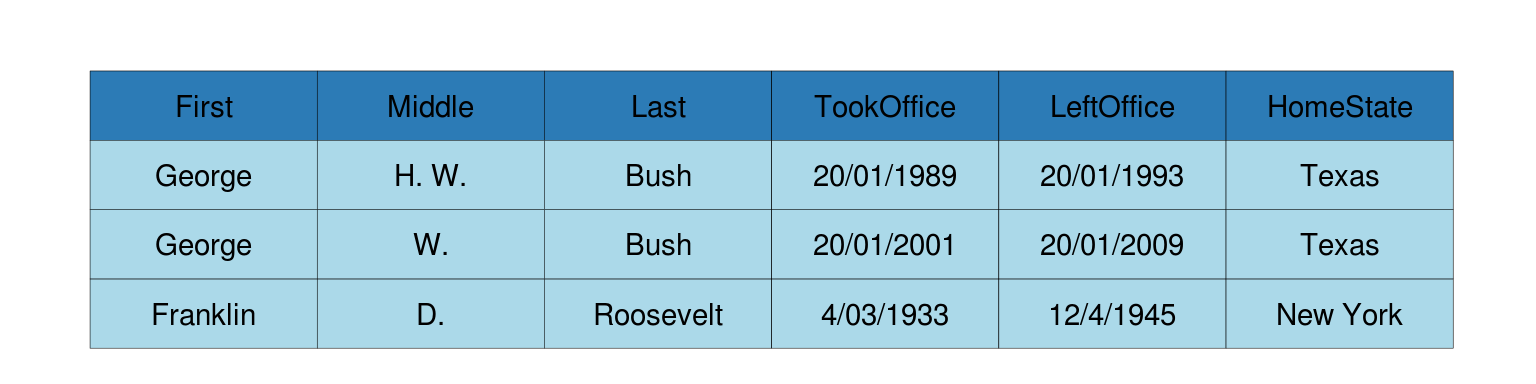
\includegraphics{tidydata_tutorial_files/figure-latex/unnamed-chunk-51-1.pdf}
\item
  Merge the two datasets so that it includes ALL the observations from
  both the datasets. Some \texttt{TookOffice,\ LeftOffice} and
  \texttt{HomeState} values will be \texttt{NA} and that's ok. The
  results should match the following:

  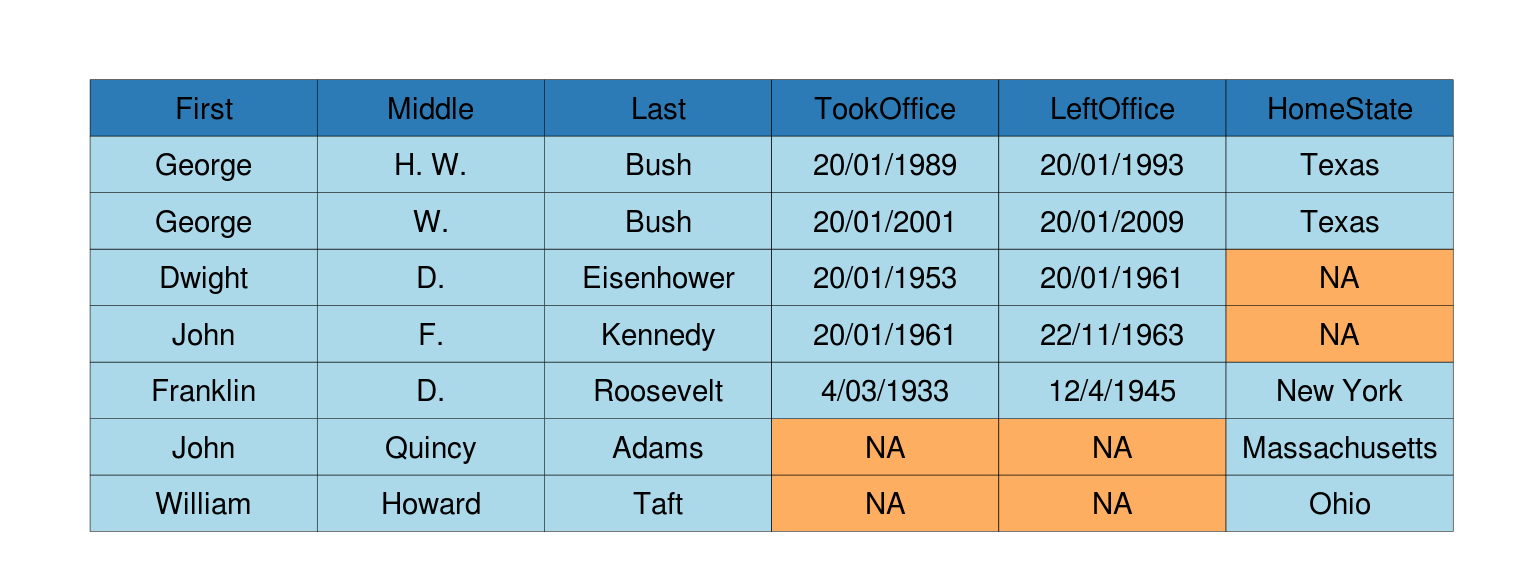
\includegraphics{tidydata_tutorial_files/figure-latex/unnamed-chunk-52-1.pdf}
\item
  Merge the two datasets so that ALL observations from the
  \texttt{presidents} datasets are included. Some \texttt{HomeState}
  values will be \texttt{NA} and that's ok. The results should match the
  following:

  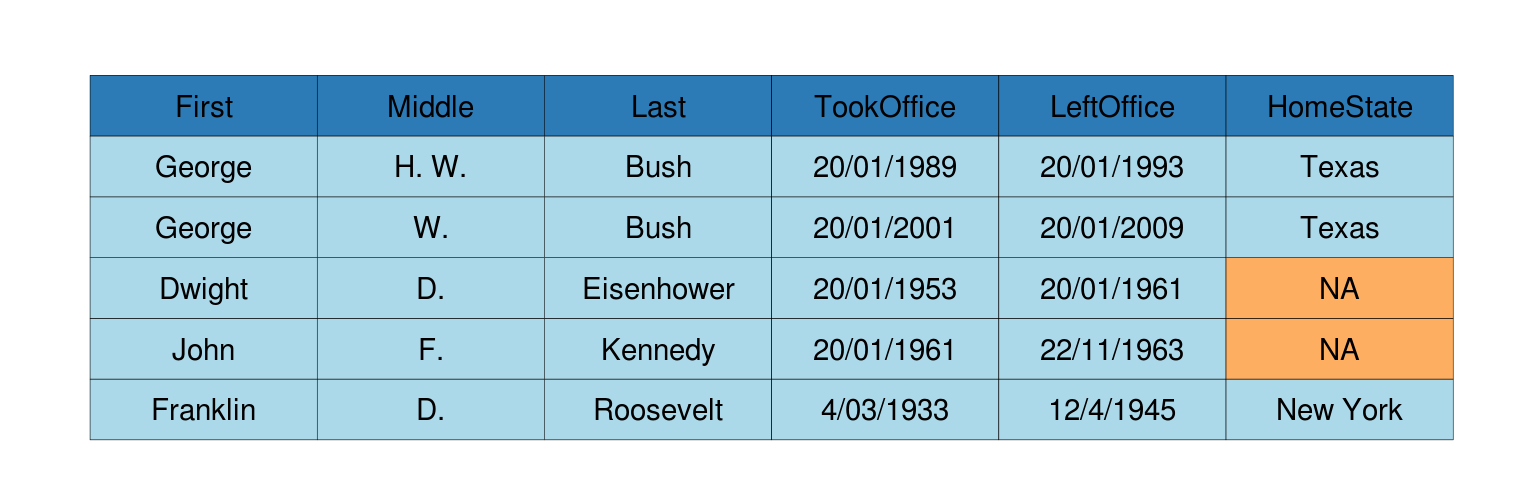
\includegraphics{tidydata_tutorial_files/figure-latex/unnamed-chunk-53-1.pdf}
\item
  Merge the two datasets so that ALL observations from the
  \texttt{presidents\_home} datasets are included. Some
  \texttt{TookOffice} and \texttt{LeftOffice} values will be \texttt{NA}
  and that's ok. The results should match the following:

  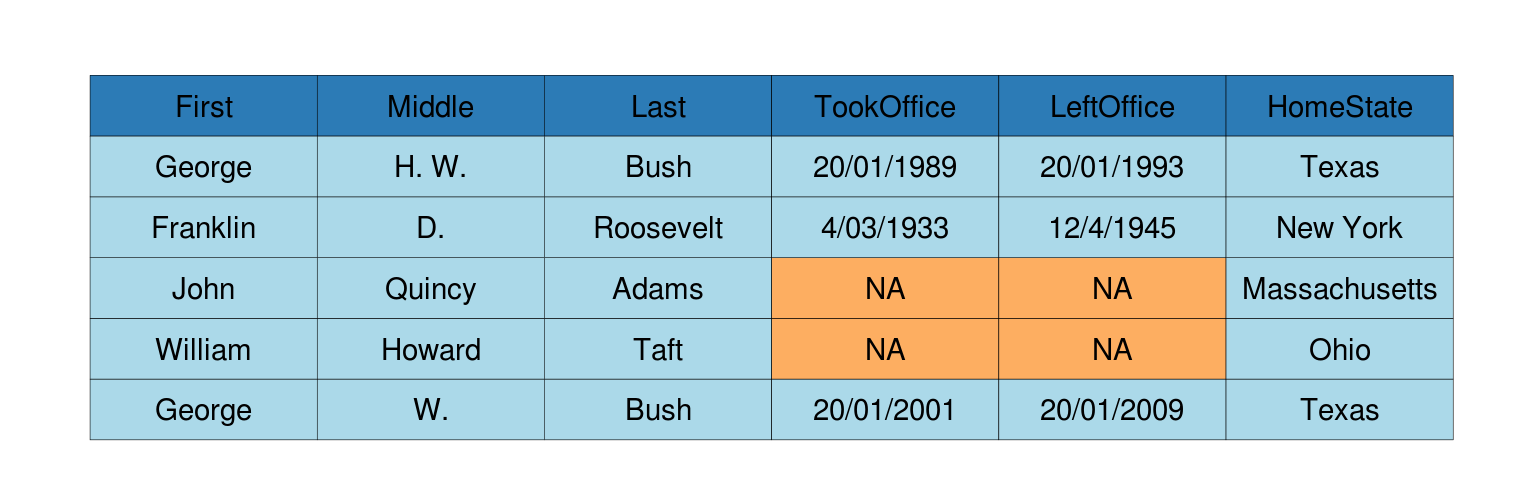
\includegraphics{tidydata_tutorial_files/figure-latex/unnamed-chunk-54-1.pdf}
\end{enumerate}

\section{Reshaping}\label{reshaping}

It's fairly common for datasets from public sources to come in formats
that need to be reshaped. The World Development Indicators (WDI) is one
such dataset that requires reshaping before we can analyse it. Let's go
over the steps to see how we can reshape the WDI dataset.

Let's start by loading the \texttt{tidyverse} package first.

\begin{Shaded}
\begin{Highlighting}[]
\KeywordTok{library}\NormalTok{(tidyverse)}
\end{Highlighting}
\end{Shaded}

Clear everything to make sure there's nothing leftover in our
environment

\begin{Shaded}
\begin{Highlighting}[]
\KeywordTok{rm}\NormalTok{(}\DataTypeTok{list =} \KeywordTok{ls}\NormalTok{())}
\end{Highlighting}
\end{Shaded}

We're using a small sample of the WDI dataset here to simplify the
tasks. Let's load the dataset and see what it looks like.

\begin{Shaded}
\begin{Highlighting}[]
\NormalTok{wdi <-}\StringTok{ }\KeywordTok{read_csv}\NormalTok{(}\StringTok{"https://raw.githubusercontent.com/altaf-ali/tidydata_tutorial/master/data/wdi.csv"}\NormalTok{, }\DataTypeTok{na =} \StringTok{".."}\NormalTok{)}

\NormalTok{wdi}
\end{Highlighting}
\end{Shaded}

\begin{verbatim}
# A tibble: 5 x 7
      `¬Series.Name`    Series.Code Country.Name Country.Code X1995.YR1995
               <chr>          <chr>        <chr>        <chr>        <dbl>
1 Maternal mortality    SH.STA.MMRT       France          FRA    15.000000
2 Maternal mortality    SH.STA.MMRT        Spain          ESP     6.000000
3 Maternal mortality    SH.STA.MMRT                                     NA
4 Health expenditure SH.XPD.TOTL.ZS       France          FRA    10.355906
5 Health expenditure SH.XPD.TOTL.ZS        Spain          ESP     7.444592
# ... with 2 more variables: X2000.YR2000 <dbl>, X2005.YR2005 <dbl>
\end{verbatim}

But ideally, we'd like our data to look something like this:

\begin{verbatim}
# A tibble: 6 x 5
  CountryCode CountryName  Year MaternalMortality HealthExpenditure
        <chr>       <chr> <dbl>             <dbl>             <dbl>
1         ESP       Spain  1995                 6          7.444592
2         ESP       Spain  2000                 5          7.214756
3         ESP       Spain  2005                 5          8.288271
4         FRA      France  1995                15         10.355906
5         FRA      France  2000                12         10.084833
6         FRA      France  2005                10         10.932626
\end{verbatim}

We can see that some country names and codes are blank, so let's get rid
of them first

\begin{Shaded}
\begin{Highlighting}[]
\NormalTok{wdi %>%}
\StringTok{  }\KeywordTok{filter}\NormalTok{(Country.Code !=}\StringTok{ ""}\NormalTok{) }
\end{Highlighting}
\end{Shaded}

\begin{verbatim}
# A tibble: 4 x 7
      `¬Series.Name`    Series.Code Country.Name Country.Code X1995.YR1995
               <chr>          <chr>        <chr>        <chr>        <dbl>
1 Maternal mortality    SH.STA.MMRT       France          FRA    15.000000
2 Maternal mortality    SH.STA.MMRT        Spain          ESP     6.000000
3 Health expenditure SH.XPD.TOTL.ZS       France          FRA    10.355906
4 Health expenditure SH.XPD.TOTL.ZS        Spain          ESP     7.444592
# ... with 2 more variables: X2000.YR2000 <dbl>, X2005.YR2005 <dbl>
\end{verbatim}

So far so good. Note that we're not making any changes yet so we can
just add one function at a time to the pipeline and check the results.
Once we're satisfied with the results we save them to a variable.

We need to gather all columns that start with ``X'' that contain
per-year values for each series (for example X1960..YR1960)

\begin{Shaded}
\begin{Highlighting}[]
\NormalTok{wdi %>%}
\StringTok{  }\KeywordTok{filter}\NormalTok{(Country.Code !=}\StringTok{ ""}\NormalTok{) %>%}\StringTok{ }
\StringTok{  }\KeywordTok{gather}\NormalTok{(Year, Value, }\KeywordTok{starts_with}\NormalTok{(}\StringTok{"X"}\NormalTok{))}
\end{Highlighting}
\end{Shaded}

\begin{verbatim}
# A tibble: 12 x 6
       `¬Series.Name`    Series.Code Country.Name Country.Code
                <chr>          <chr>        <chr>        <chr>
 1 Maternal mortality    SH.STA.MMRT       France          FRA
 2 Maternal mortality    SH.STA.MMRT        Spain          ESP
 3 Health expenditure SH.XPD.TOTL.ZS       France          FRA
 4 Health expenditure SH.XPD.TOTL.ZS        Spain          ESP
 5 Maternal mortality    SH.STA.MMRT       France          FRA
 6 Maternal mortality    SH.STA.MMRT        Spain          ESP
 7 Health expenditure SH.XPD.TOTL.ZS       France          FRA
 8 Health expenditure SH.XPD.TOTL.ZS        Spain          ESP
 9 Maternal mortality    SH.STA.MMRT       France          FRA
10 Maternal mortality    SH.STA.MMRT        Spain          ESP
11 Health expenditure SH.XPD.TOTL.ZS       France          FRA
12 Health expenditure SH.XPD.TOTL.ZS        Spain          ESP
# ... with 2 more variables: Year <chr>, Value <dbl>
\end{verbatim}

Now all values are in the \texttt{Value} column, so we need to spread
them out to individual columns based on the \texttt{Series.Code}. We
have to make sure that we only keep the columns that make the
country-year observations unique. We use \texttt{select()} to keep
\texttt{Country.Code}, \texttt{Country.Name}, \texttt{Year}, plus the
two columns (\texttt{Series.Code} and \texttt{Value}) that will make up
the key-value pair for the \texttt{spread()} function.

\begin{Shaded}
\begin{Highlighting}[]
\NormalTok{wdi %>%}
\StringTok{  }\KeywordTok{filter}\NormalTok{(Country.Code !=}\StringTok{ ""}\NormalTok{) %>%}\StringTok{ }
\StringTok{  }\KeywordTok{gather}\NormalTok{(Year, Value, }\KeywordTok{starts_with}\NormalTok{(}\StringTok{"X"}\NormalTok{)) %>%}\StringTok{ }
\StringTok{  }\KeywordTok{select}\NormalTok{(Country.Code, Country.Name, Year, Series.Code, Value) %>%}
\StringTok{  }\KeywordTok{spread}\NormalTok{(Series.Code, Value) }
\end{Highlighting}
\end{Shaded}

\begin{verbatim}
# A tibble: 6 x 5
  Country.Code Country.Name         Year SH.STA.MMRT SH.XPD.TOTL.ZS
*        <chr>        <chr>        <chr>       <dbl>          <dbl>
1          ESP        Spain X1995.YR1995           6       7.444592
2          ESP        Spain X2000.YR2000           5       7.214756
3          ESP        Spain X2005.YR2005           5       8.288271
4          FRA       France X1995.YR1995          15      10.355906
5          FRA       France X2000.YR2000          12      10.084833
6          FRA       France X2005.YR2005          10      10.932626
\end{verbatim}

It looks good, so we can rename the variables to something meaningful.

\begin{Shaded}
\begin{Highlighting}[]
\NormalTok{wdi %>%}
\StringTok{  }\KeywordTok{filter}\NormalTok{(Country.Code !=}\StringTok{ ""}\NormalTok{) %>%}\StringTok{ }
\StringTok{  }\KeywordTok{gather}\NormalTok{(Year, Value, }\KeywordTok{starts_with}\NormalTok{(}\StringTok{"X"}\NormalTok{)) %>%}\StringTok{ }
\StringTok{  }\KeywordTok{select}\NormalTok{(Country.Code, Country.Name, Year, Series.Code, Value) %>%}
\StringTok{  }\KeywordTok{spread}\NormalTok{(Series.Code, Value) %>%}\StringTok{ }
\StringTok{  }\KeywordTok{rename}\NormalTok{(}\DataTypeTok{CountryName =} \NormalTok{Country.Name,}
         \DataTypeTok{CountryCode =} \NormalTok{Country.Code,}
         \DataTypeTok{MaternalMortality =} \NormalTok{SH.STA.MMRT,}
         \DataTypeTok{HealthExpenditure =} \NormalTok{SH.XPD.TOTL.ZS)}
\end{Highlighting}
\end{Shaded}

\begin{verbatim}
# A tibble: 6 x 5
  CountryCode CountryName         Year MaternalMortality HealthExpenditure
*       <chr>       <chr>        <chr>             <dbl>             <dbl>
1         ESP       Spain X1995.YR1995                 6          7.444592
2         ESP       Spain X2000.YR2000                 5          7.214756
3         ESP       Spain X2005.YR2005                 5          8.288271
4         FRA      France X1995.YR1995                15         10.355906
5         FRA      France X2000.YR2000                12         10.084833
6         FRA      France X2005.YR2005                10         10.932626
\end{verbatim}

Now we just need to extract the 4-digit year from the \texttt{Year}
column. The \texttt{Year} column is formatted as \texttt{X1995.YR1995}
which means that the 4-digits for the year are in position
\texttt{2},\texttt{3},\texttt{4}, and \texttt{5}. We can use the
\texttt{substring()} function to take all the characters from position
\texttt{2} to \texttt{5} and assign it back to the \texttt{Year} column.

Since this is the last step we might as well assign the results to a new
variable.

\begin{Shaded}
\begin{Highlighting}[]
\NormalTok{wdi_long <-}\StringTok{ }\NormalTok{wdi %>%}
\StringTok{  }\KeywordTok{filter}\NormalTok{(Country.Code !=}\StringTok{ ""}\NormalTok{) %>%}\StringTok{ }
\StringTok{  }\KeywordTok{gather}\NormalTok{(Year, Value, }\KeywordTok{starts_with}\NormalTok{(}\StringTok{"X"}\NormalTok{)) %>%}\StringTok{ }
\StringTok{  }\KeywordTok{select}\NormalTok{(Country.Code, Country.Name, Year, Series.Code, Value) %>%}
\StringTok{  }\KeywordTok{spread}\NormalTok{(Series.Code, Value) %>%}\StringTok{ }
\StringTok{  }\KeywordTok{rename}\NormalTok{(}\DataTypeTok{CountryName =} \NormalTok{Country.Name,}
         \DataTypeTok{CountryCode =} \NormalTok{Country.Code,}
         \DataTypeTok{MaternalMortality =} \NormalTok{SH.STA.MMRT,}
         \DataTypeTok{HealthExpenditure =} \NormalTok{SH.XPD.TOTL.ZS) %>%}
\StringTok{  }\KeywordTok{mutate}\NormalTok{(}\DataTypeTok{Year =} \KeywordTok{as.numeric}\NormalTok{(}\KeywordTok{substring}\NormalTok{(Year, }\DecValTok{2}\NormalTok{, }\DecValTok{5}\NormalTok{)))}

\NormalTok{wdi_long }
\end{Highlighting}
\end{Shaded}

\begin{verbatim}
# A tibble: 6 x 5
  CountryCode CountryName  Year MaternalMortality HealthExpenditure
        <chr>       <chr> <dbl>             <dbl>             <dbl>
1         ESP       Spain  1995                 6          7.444592
2         ESP       Spain  2000                 5          7.214756
3         ESP       Spain  2005                 5          8.288271
4         FRA      France  1995                15         10.355906
5         FRA      France  2000                12         10.084833
6         FRA      France  2005                10         10.932626
\end{verbatim}

You can assign it back to \texttt{wdi} if you want, but we're using a
different name in case we make a mistake and have to start again. This
way we would've have to reload the file all over again.

\end{document}
